
%使用XeLaTeX编译
%版权所有,翻版必究
%本文件由程序自动生成,任何修改将被覆盖
%2019 年 01 月 23 日




%导引

\FloatBarrier
\section{
导引
}\label{c000019s01}


%%%%%%%%%%%%%%%%%%%%%%%%%%%%%%%导引

\FloatBarrier
\subsection{
使用QtCreator快速创建模型
}\label{c000019s01s01}


无论是对于初学者还是老手,
通过继承自QAbstractItemModel
创建自己的模型都是一件麻烦的事。

所幸的是QtCreator可以帮助我们快速的
创建出我们所需的模型的架构。

\begin{enumerate}

\item 如\figurename\ \ref{p000044}所示。
在项目名称单击右键,选择“Add New\ldots”。
\FloatBarrier
%begin图片
\begin{figure}[htb] %浮动体 here and top ...
%there must use marginnote ...
\marginnote{\setlength\fboxsep{2pt}\fbox{\footnotesize{\kaishu\figurename\,}\footnotesize{\ref{p000044}}}}\centering %中心对齐
\setlength\fboxsep{0pt}\fcolorbox[rgb]{0,0,0}{0,0,0}{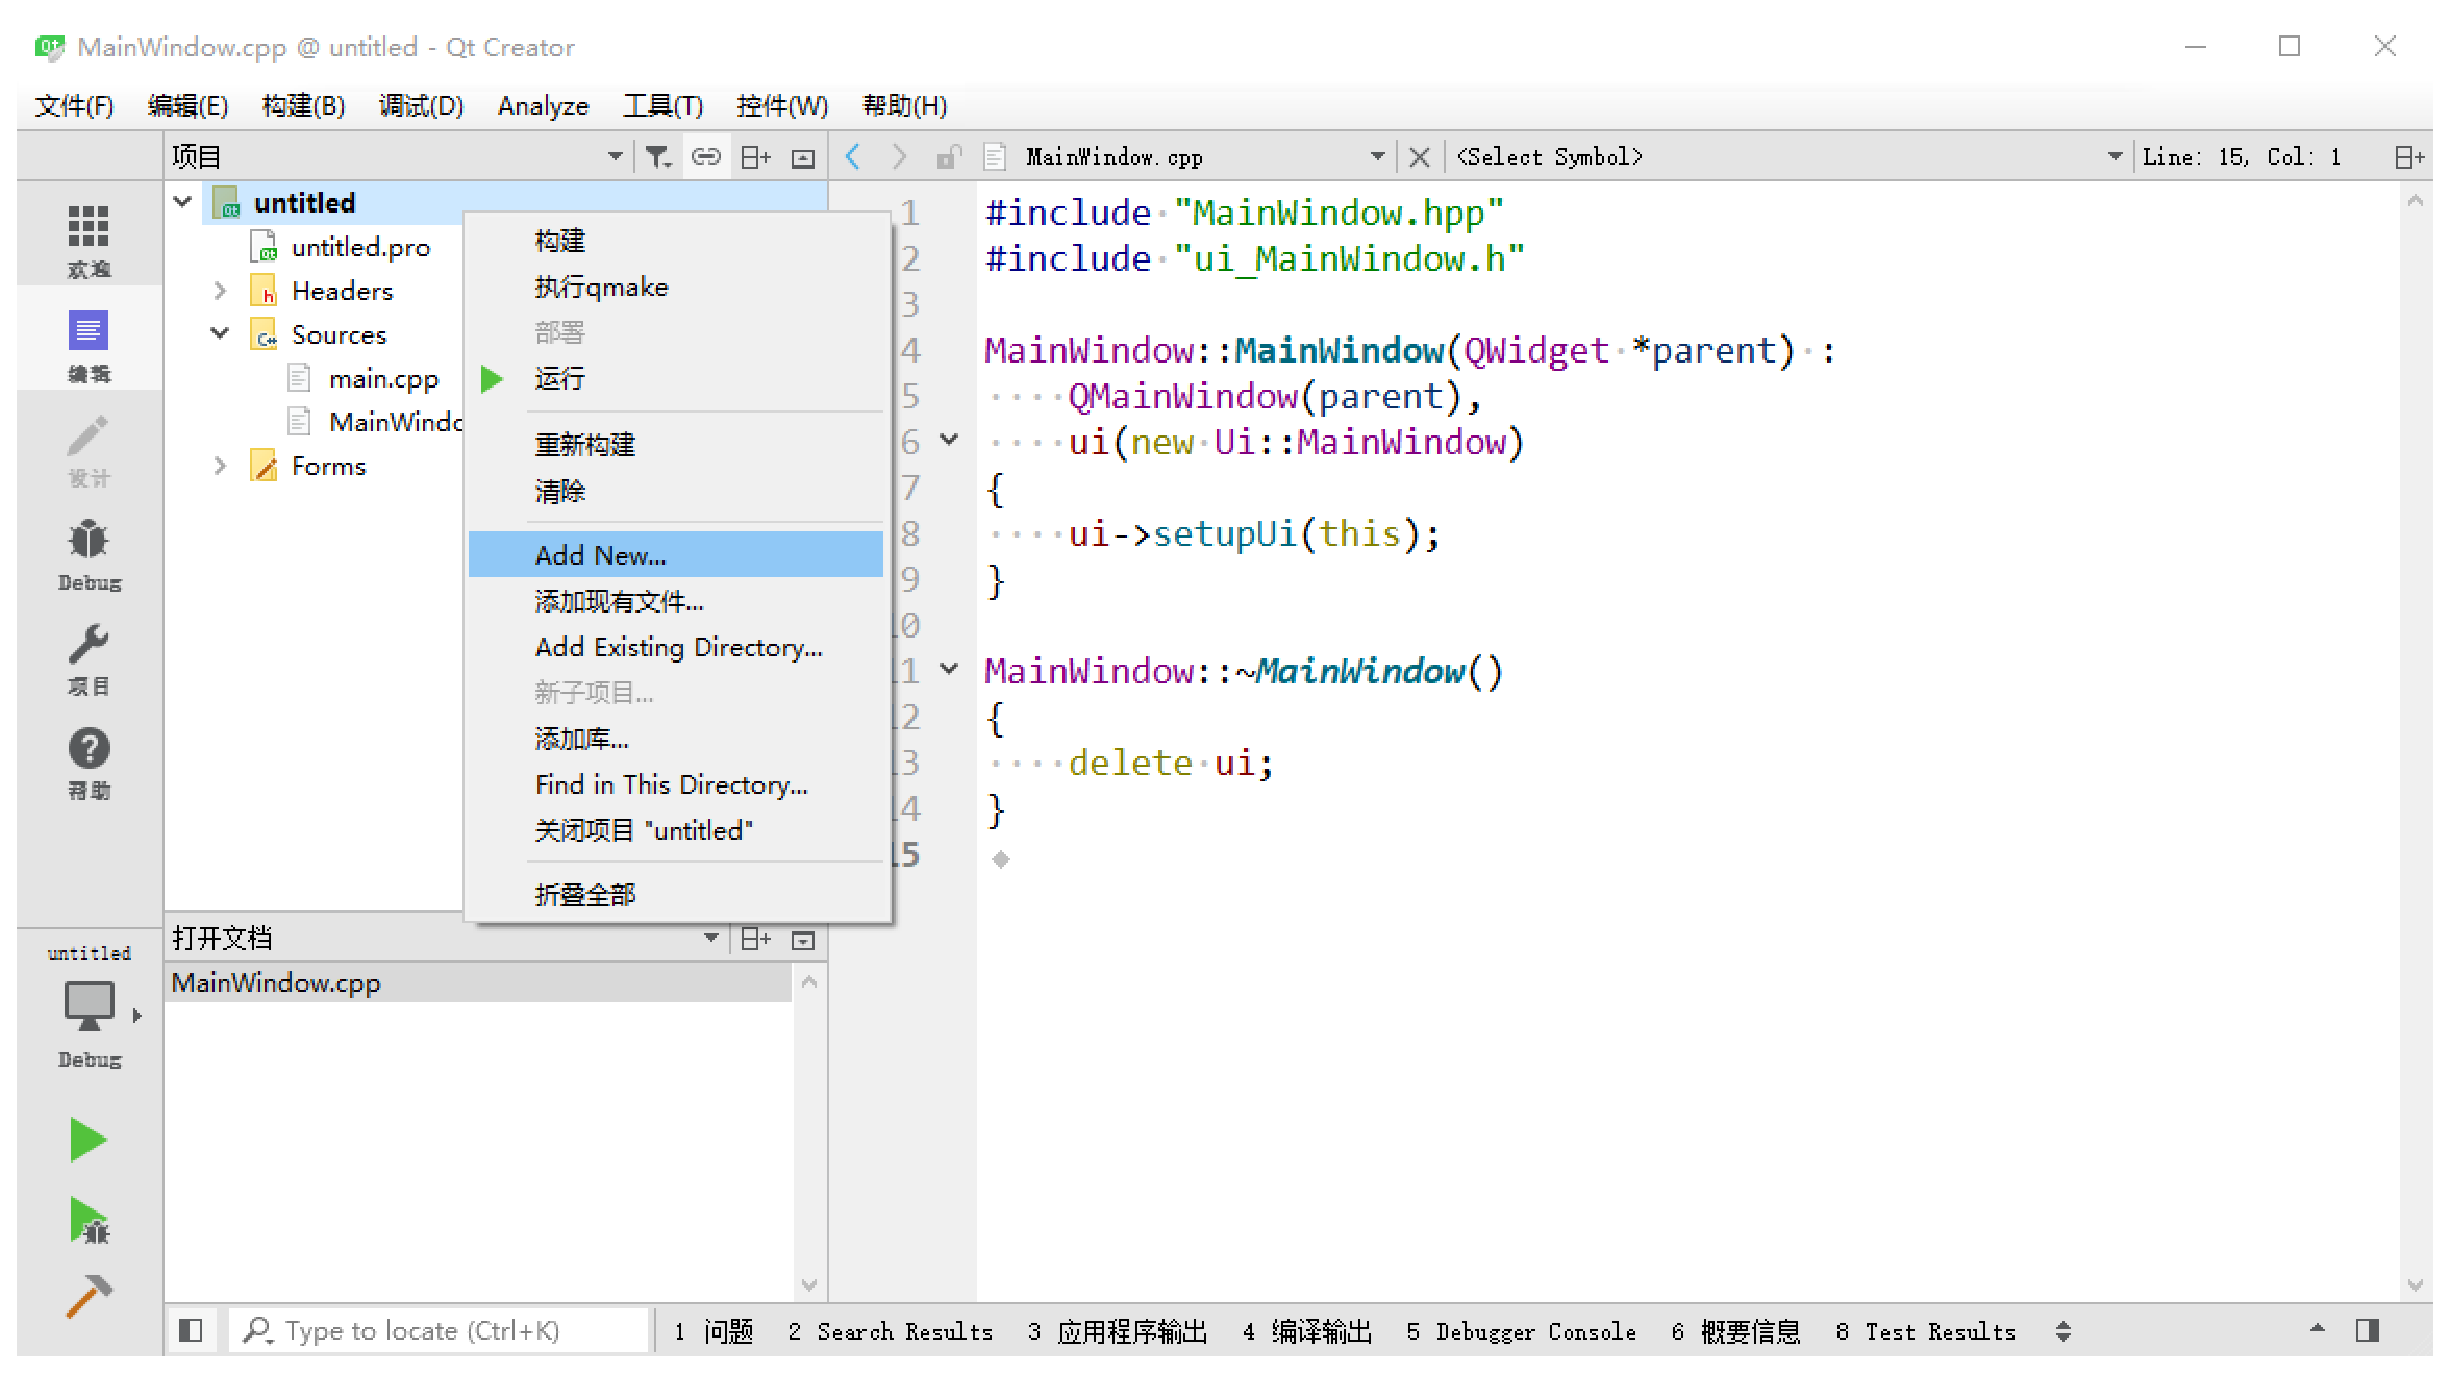
\includegraphics[width=0.95\textwidth]{the_book_image/p000044.eps}} %图片路径
\caption{使用QtCreator创建模型} %标题
\label{p000044} %索引
\end{figure}
%end图片


\item 如\figurename\ \ref{p000045}所示。
选择“Qt Item Model”模板。
\FloatBarrier
%begin图片
\begin{figure}[htb] %浮动体 here and top ...
%there must use marginnote ...
\marginnote{\setlength\fboxsep{2pt}\fbox{\footnotesize{\kaishu\figurename\,}\footnotesize{\ref{p000045}}}}\centering %中心对齐
\setlength\fboxsep{0pt}\fcolorbox[rgb]{0,0,0}{0,0,0}{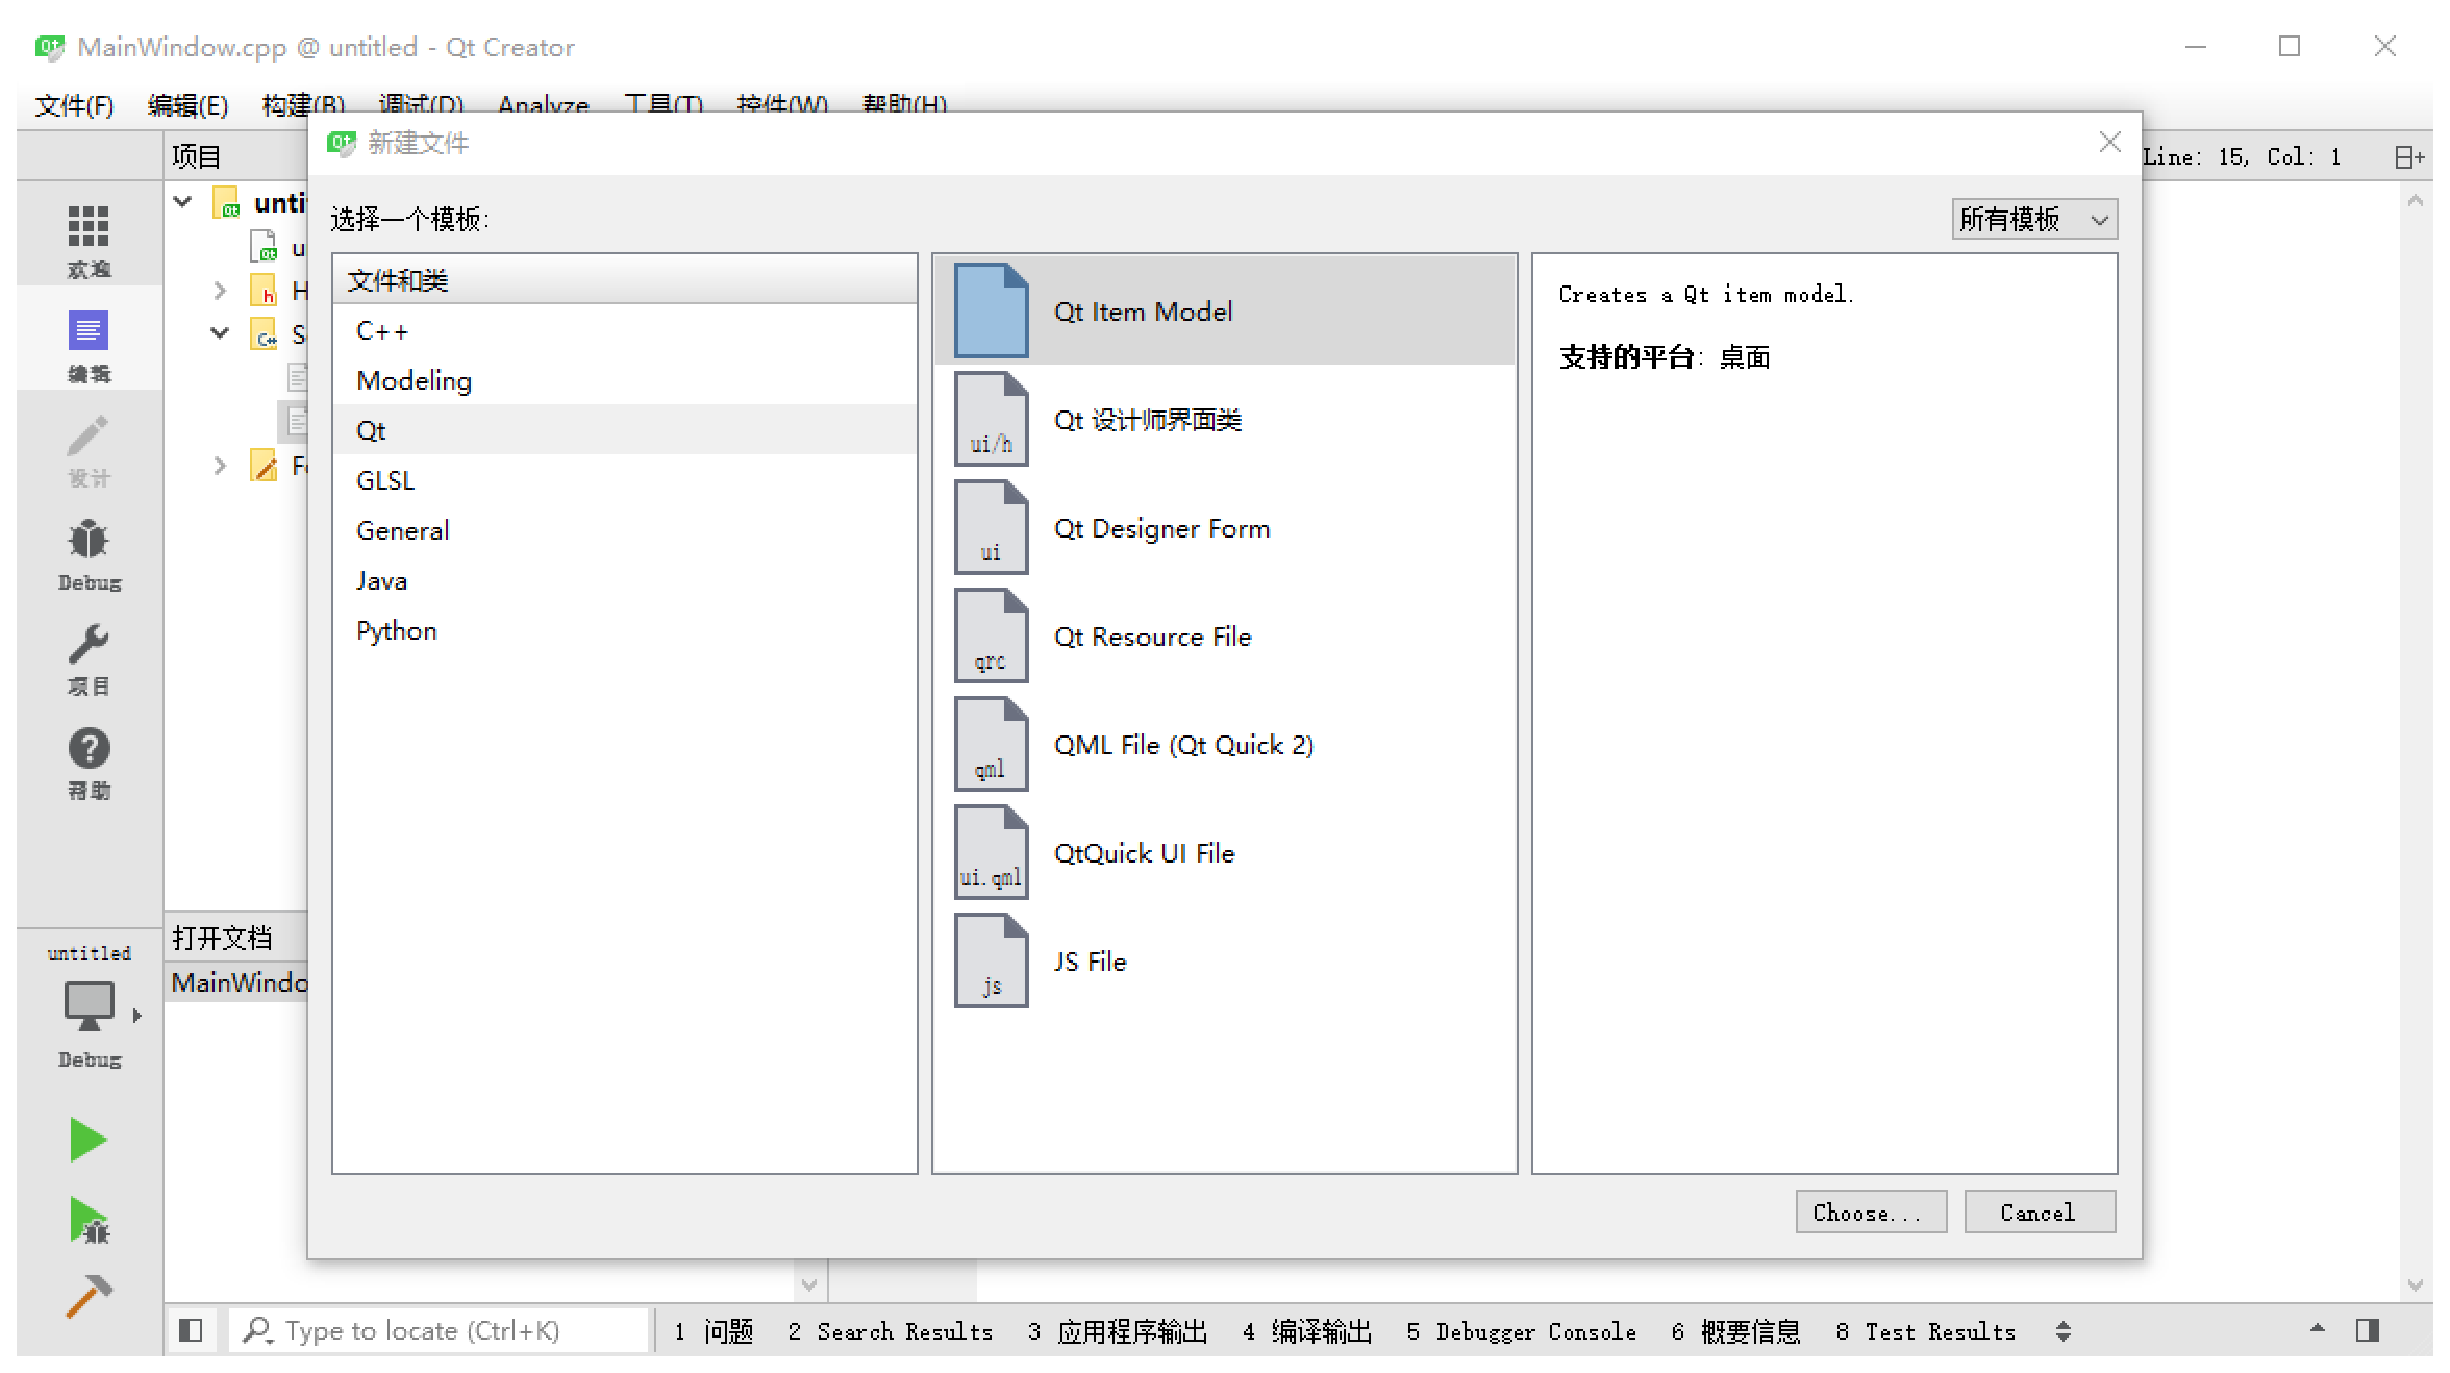
\includegraphics[width=0.95\textwidth]{the_book_image/p000045.eps}} %图片路径
\caption{使用QtCreator创建模型} %标题
\label{p000045} %索引
\end{figure}
%end图片


\item 如\figurename\ \ref{p000046}所示。
输入类名,并选择所需功能。
如果没有选择任何功能,则创建一个只读的模型。
\begin{tabbing}
\textbullet\ Rows and columns can be removed \hspace{2em} \= MMM \kill
\textbullet\ Customize header row\>
自定义标题 \\
\textbullet\ Items are editable \>
数据元素可编辑 \\
\textbullet\ Rows and columns can be added \>
可以添加行或列 \\
\textbullet\ Rows and columns can be removed \>
可以删除行或列 \\
\textbullet\ Fetch data dynamically \>
下拉获得更多数据 \\
\end{tabbing}

\FloatBarrier
%begin图片
\begin{figure}[htb] %浮动体 here and top ...
%there must use marginnote ...
\marginnote{\setlength\fboxsep{2pt}\fbox{\footnotesize{\kaishu\figurename\,}\footnotesize{\ref{p000046}}}}\centering %中心对齐
\setlength\fboxsep{0pt}\fcolorbox[rgb]{0,0,0}{0,0,0}{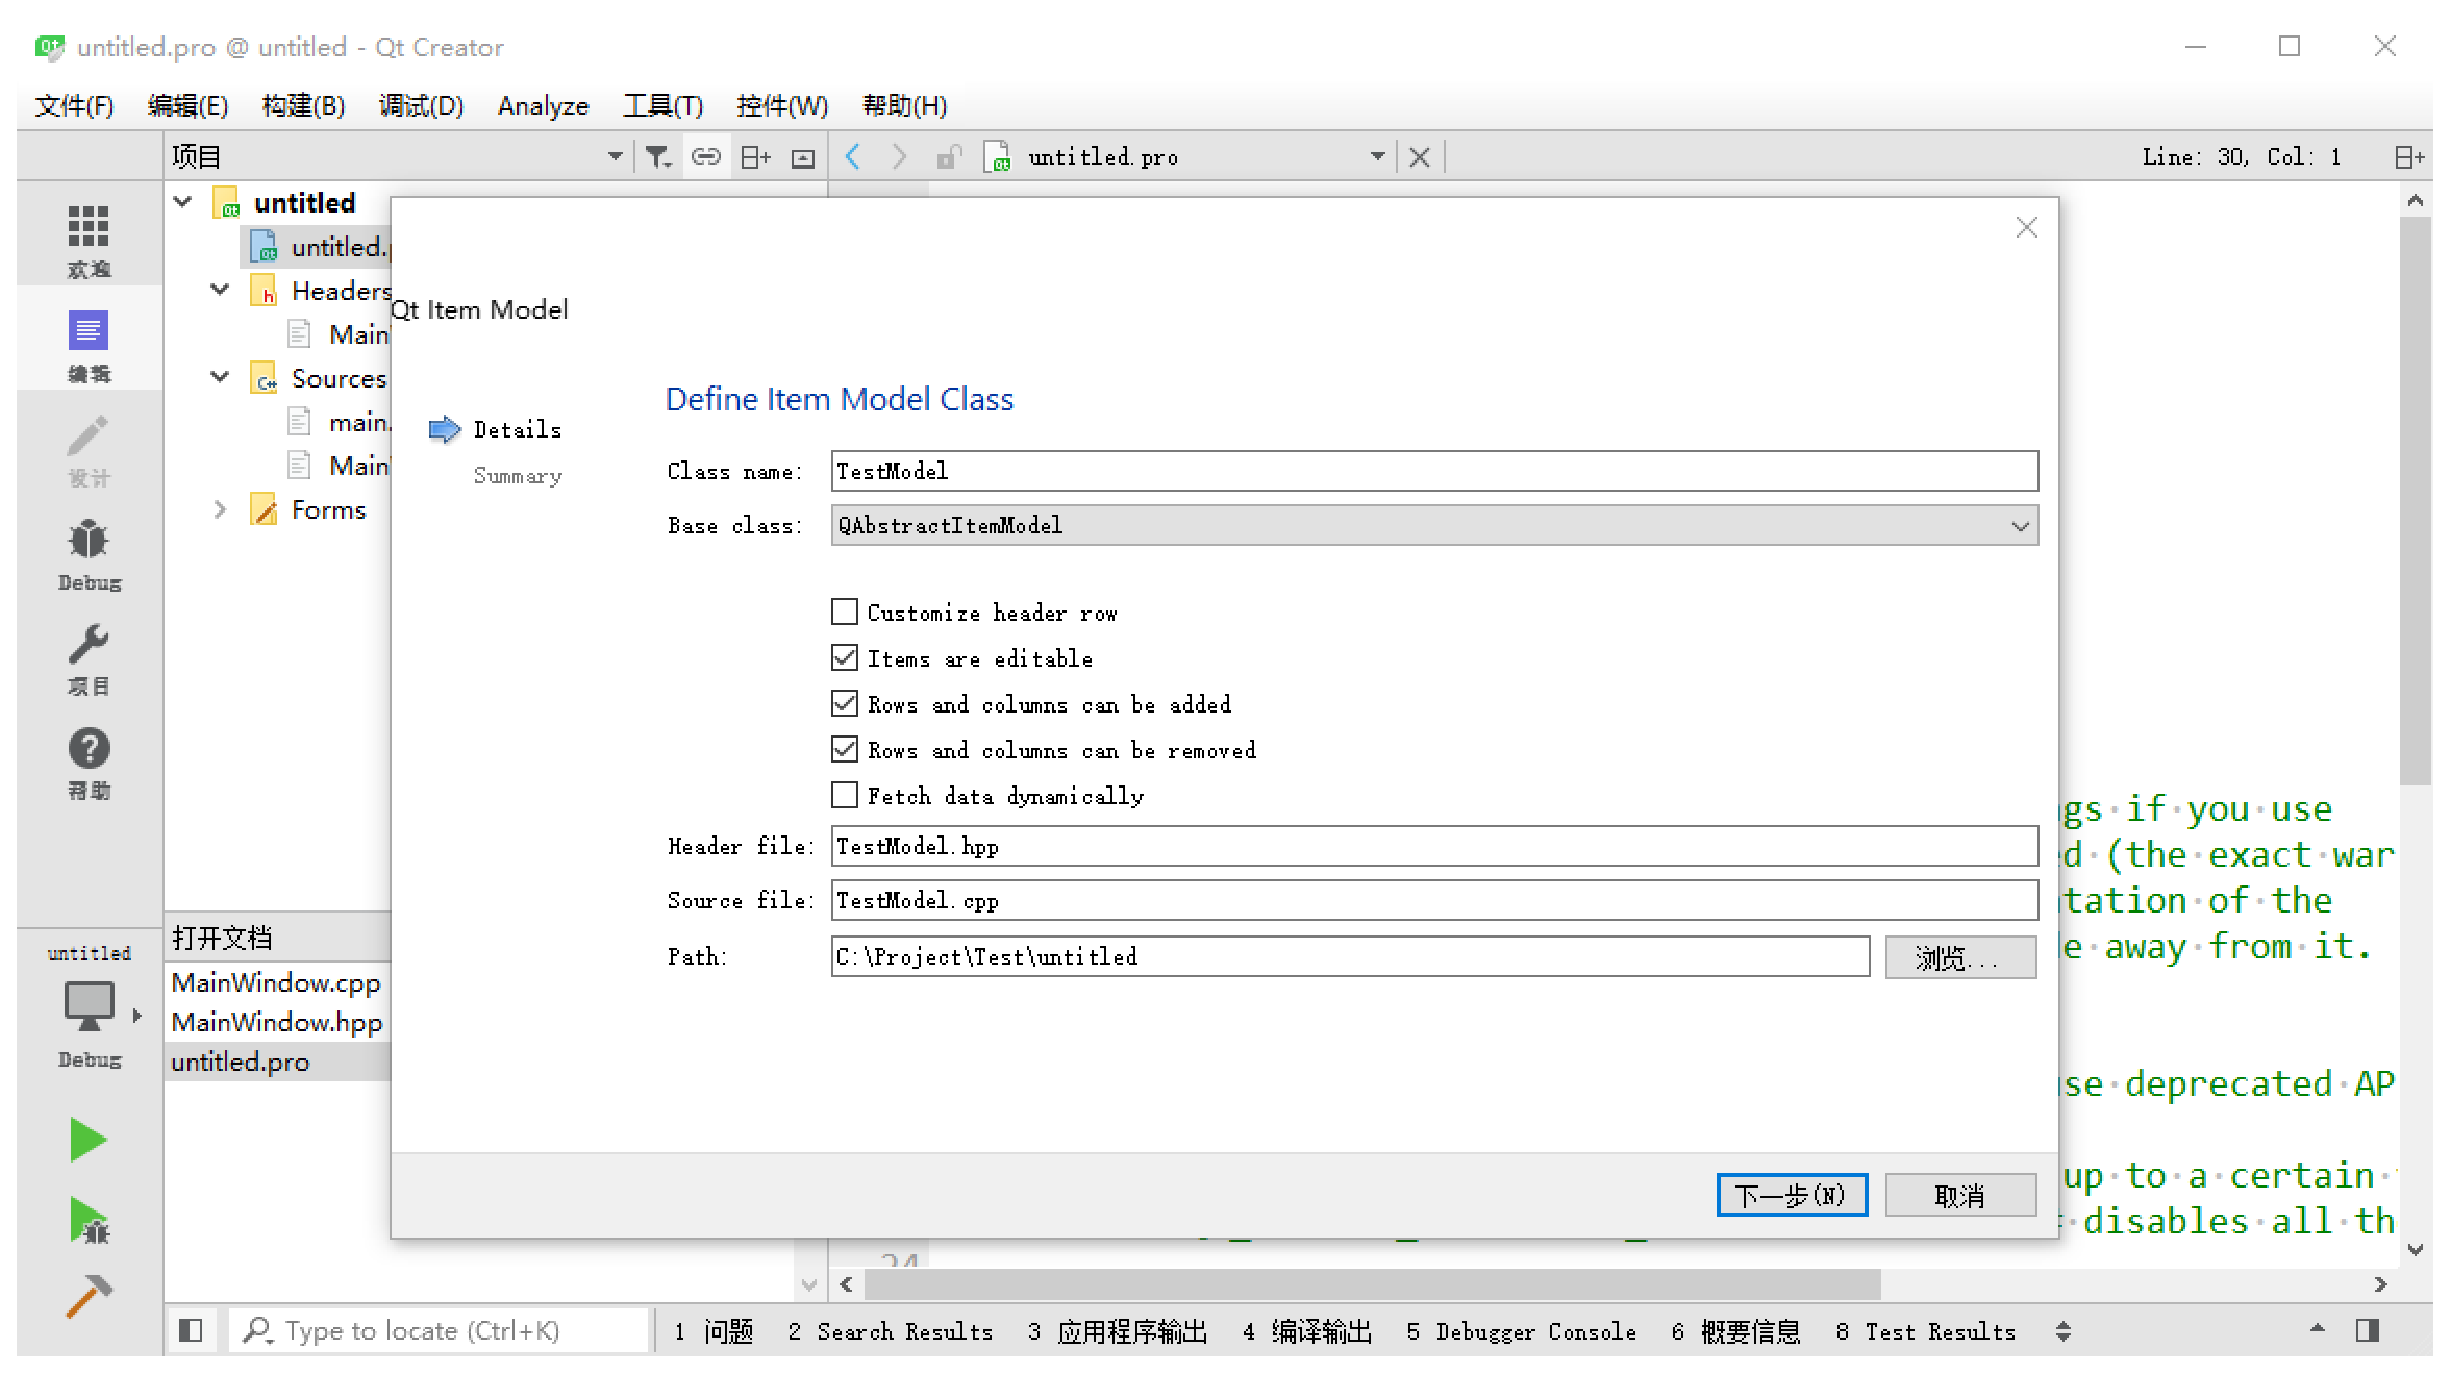
\includegraphics[width=0.95\textwidth]{the_book_image/p000046.eps}} %图片路径
\caption{使用QtCreator创建模型} %标题
\label{p000046} %索引
\end{figure}
%end图片


\end{enumerate}

%%%%%%%%%%%%%%%%%%%%%%%%%%%%%%%模型与地址
\FloatBarrier
\subsection{
模型与地址
}\label{c000019s01s03}


%begin图片
\begin{figure}[htb] %浮动体 here and top ...
%there must use marginnote ...
\marginnote{\setlength\fboxsep{2pt}\fbox{\footnotesize{\kaishu\figurename\,}\footnotesize{\ref{p000048}}}}\centering %中心对齐
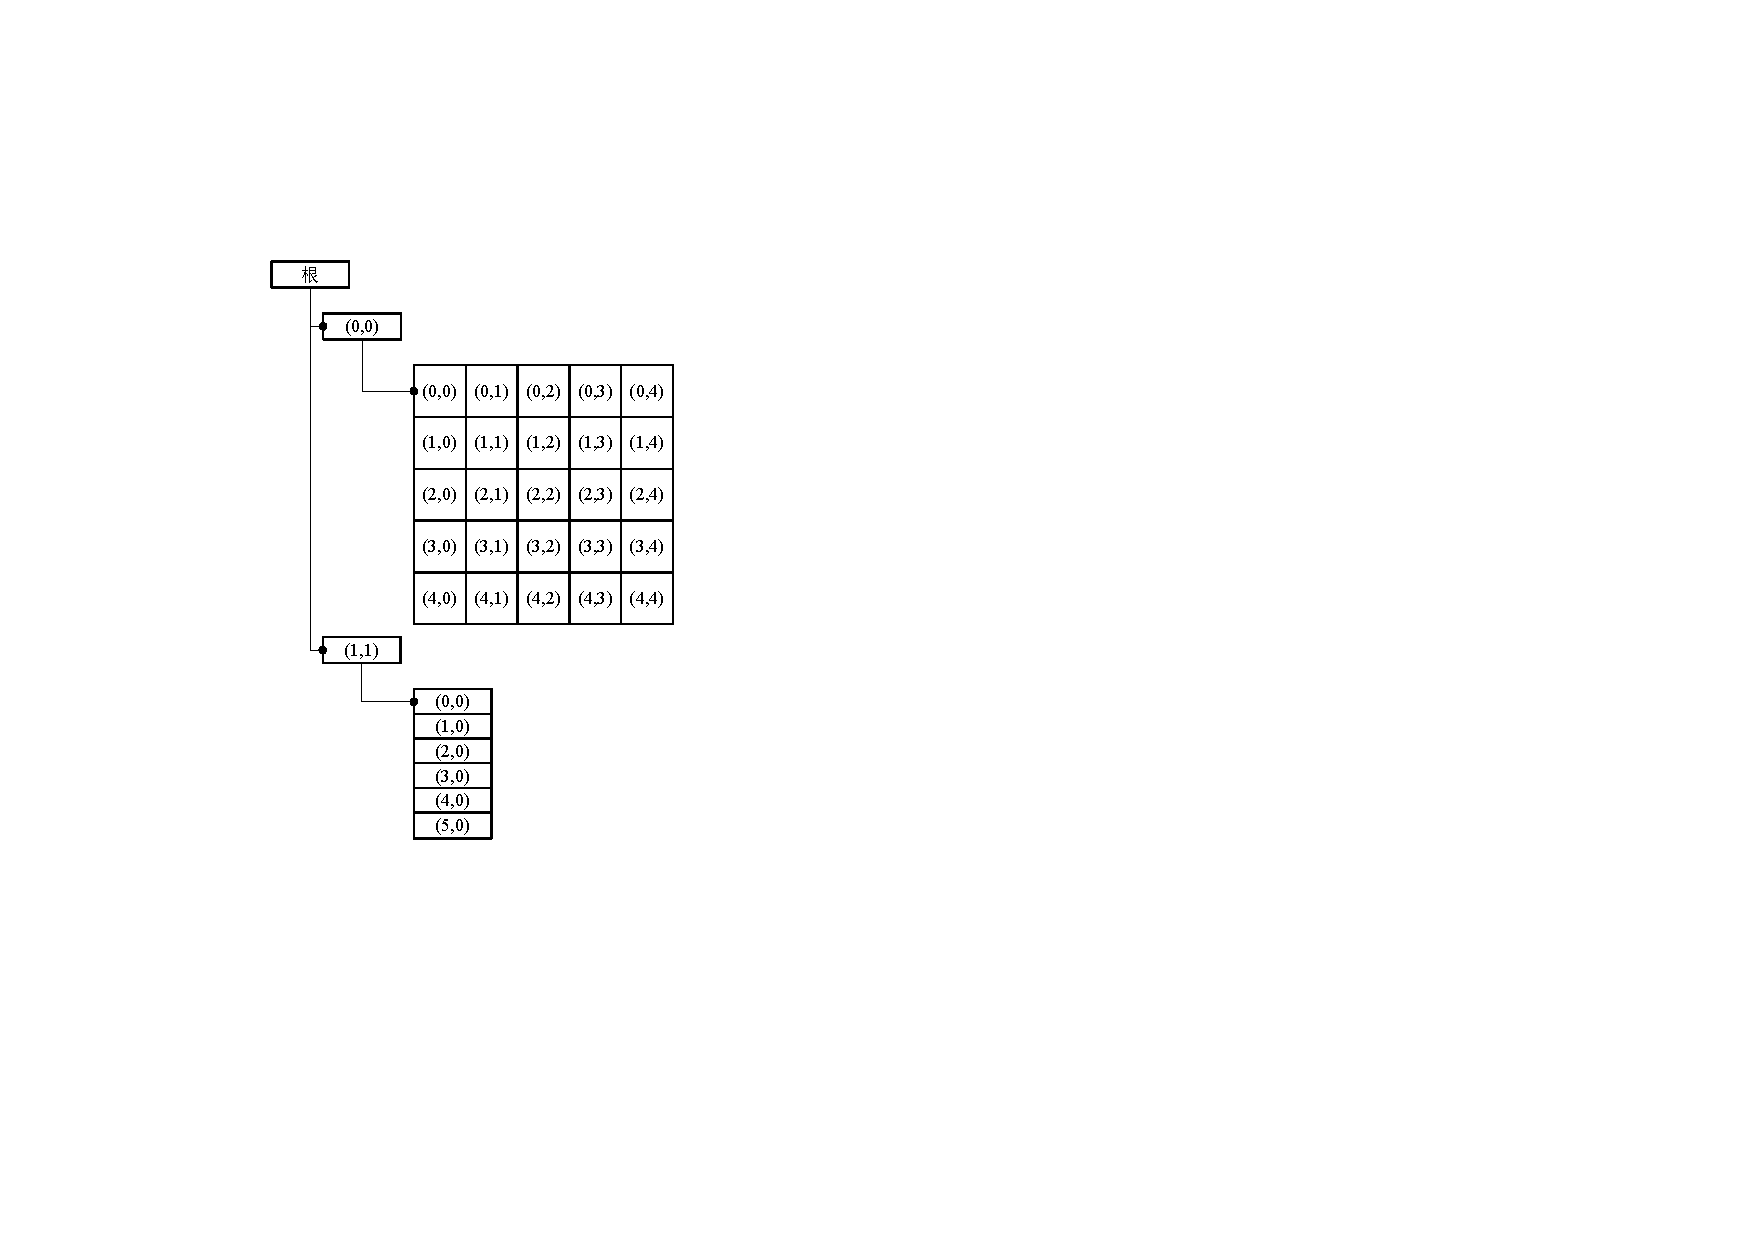
\includegraphics[width=7.5cm]{chapter10/images/ModelAndIndex.pdf} %图片路径
\caption{Qt Model模型} %标题
\label{p000048} %索引
\end{figure}
%end图片


如\figurename\ \ref{p000048},展示了一个深度
为2的一棵QAbstractItemModel树。

%%%%%%%%%%%%%%%%%%%%%%%%%%%%%%%QAbstractItemModel根
\FloatBarrier
\subsubsection{
根
}\label{c000019s01s03s01}


%%%%%%%%%%%%%%%%%%%%%%%%%%%%%%%QAbstractItemModel重要函数解析
\FloatBarrier
\subsection{
QAbstractItemModel重要函数解析
}\label{c000019s01s02}



\begin{comment}

QHash<int, QByteArray> roleNames() const

Qt::ItemFlags flags(const QModelIndex &index) const

QModelIndex index(int row, int column, const QModelIndex &parent) const
QModelIndex parent(const QModelIndex &index) const

int rowCount(const QModelIndex &parent) const
int columnCount(const QModelIndex &parent) const

QVariant data(const QModelIndex &index, int role) const
bool setData(const QModelIndex &index, const QVariant &value, int role)

bool insertRows(int row, int count, const QModelIndex &parent)
bool insertColumns(int column, int count, const QModelIndex &parent)

bool removeRows(int row, int count, const QModelIndex &parent)
bool removeColumns(int column, int count, const QModelIndex &parent)

\end{comment}




%begin图片
\begin{figure}[htb] %浮动体 here and top ...
%there must use marginnote ...
\marginnote{\setlength\fboxsep{2pt}\fbox{\footnotesize{\kaishu\figurename\,}\footnotesize{\ref{p000047}}}}\centering %中心对齐
\setlength\fboxsep{0pt}\fcolorbox[rgb]{0,0,0}{0,0,0}{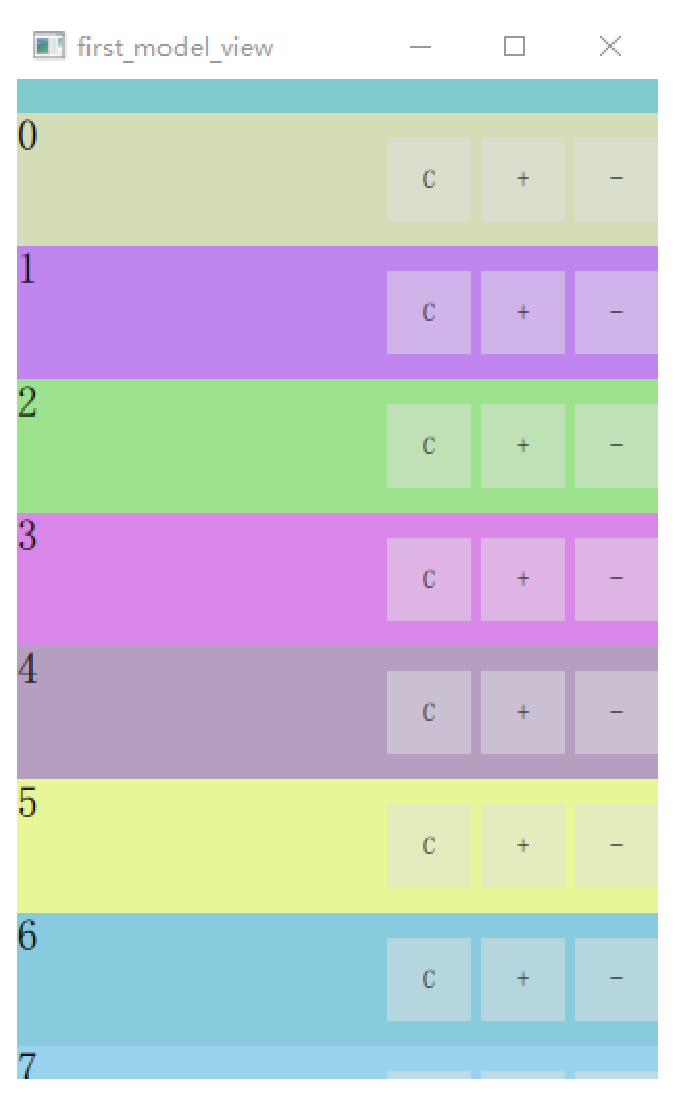
\includegraphics[height=0.75\textwidth]{the_book_image/p000047.eps}} %图片路径
\caption{List} %标题
\label{p000047} %索引
\end{figure}
%end图片


















%使用XeLaTeX编译
%版权所有,翻版必究
%本文件由程序自动生成,任何修改将被覆盖
%2019 年 01 月 23 日



